\documentclass[journal=jcisd8,manuscript=article]{achemso}
\usepackage[version=3]{mhchem}
\usepackage{microtype}
\usepackage{graphicx}
\usepackage{xurl}
\usepackage{caption}
\usepackage{orcidlink}
\usepackage{booktabs}
\usepackage{amsmath,amssymb}
\setcitestyle{super,sort&compress,comma}

\captionsetup{font=small,labelfont=bf}
\setlength{\parskip}{4pt}
\setlength{\parindent}{0pt}
\emergencystretch=1em

% Auto-generated by paper_3domain/scripts/generate_paper_artifacts.py — do not edit.
\newcommand{\MacroUvEnsMae}{17.48}
\newcommand{\MacroUvEnsRsq}{0.9221}
\newcommand{\MacroUvHoldMae}{18.50}
\newcommand{\MacroMorganMae}{24.04}
\newcommand{\MacroUvNtest}{643}
\newcommand{\MacroUvNtrain}{5{,}782}
\newcommand{\MacroUvGnnInband}{0.720 $\pm$ 0.037}
\newcommand{\MacroUvEtInband}{0.702 $\pm$ 0.025}
\newcommand{\MacroPlCompliance}{99.97}
\newcommand{\MacroPlCompliancePrior}{0.893}
\newcommand{\MacroPlValidPrior}{0.717}
\newcommand{\MacroPlValidFinal}{0.967}
\newcommand{\MacroPlInbandGnn}{0.807}
\newcommand{\MacroPlInbandPriorGnn}{0.201}
\newcommand{\MacroPlEnsMae}{20.96}
\newcommand{\MacroPlEnsRsq}{0.922}
\newcommand{\MacroCorpFailPct}{15.07}
\newcommand{\MacroCorpFailN}{1{,}110}
\newcommand{\MacroCorpN}{7{,}367}
\newcommand{\MacroCnsUniqMurcko}{0.994}
\newcommand{\MacroCnsUniqSafety}{0.266}
\newcommand{\MacroCns5ht2bNoMem}{0.551}
\newcommand{\MacroCns5ht2bMem}{0.228}
\newcommand{\MacroCnsHergNoMem}{0.959}
\newcommand{\MacroCnsHergMem}{0.750}
\newcommand{\MacroDftS1Ge380Cnt}{30}
\newcommand{\MacroDftS1Ge380Of}{46}
\newcommand{\MacroDftS1In400450Cnt}{7}
\newcommand{\MacroDftBrightCnt}{6}
\newcommand{\MacroDftConvFrac}{92.0}
\newcommand{\MacroDftMaeGnn}{83.9}
\newcommand{\MacroPlHoldInbandGnn}{0.201}
\newcommand{\MacroPlHoldInbandEt}{0.191}
\newcommand{\MacroPlHoldInbandGnnFin}{0.807}
\newcommand{\MacroPlHoldInbandEtFin}{0.522}


\title{\textbf{Compliance-Conditioned Molecular Generation Across Optical, Polymer,\\
and Central Nervous System Targets with Graph Neural Network Ensembles}}

\author{Julian M. Kleber\,\orcidlink{0000-0001-5518-0932}}
\affiliation[Independent]{Independent researcher, Berlin, Germany}

\date{November 19, 2026}

\begin{document}
\maketitle

\begin{abstract}
\noindent
Generative molecular design usually optimises a single physical or biological target while
treating regulatory bans and safety risks as an afterthought. At the same time,
reinforcement learning against a single surrogate readily exploits out-of-distribution
features or collapses onto narrow scaffolds. We evaluate a unified compliance-conditioned
generation framework that embeds explicit regulatory and safety gates directly into
REINVENT policy-gradient fine-tuning, guided by four-architecture 2D graph neural network
ensembles (\texttt{GINE}, \texttt{GATv2}, \texttt{MPNN}, and \texttt{CARATE}) and audited
by an independent ExtraTrees holdout excluded from training rewards. Across three distinct
chemical domains on a single RTX~3060 GPU, the framework resolves domain-specific failure
modes. For UV-Vis chromophores (400--450~nm), graph-ensemble rewards align training and
holdout gains above $70\%$ in-band yield across three prior seeds ($n=10{,}000$ samples per
seed) while cutting cross-seed variance nearly fourfold versus a Morgan-only reward.
For engineering polymers ($T_g$ 450--550~K), where \MacroCorpFailPct{}\% of the
curated corpus ($N=\MacroCorpN{}$) fails REACH or bisphenol-A rules, compliance-gated
generation reaches \MacroPlCompliance{}\% compliance with a fourfold increase in target-band
yield. For non-hallucinogenic central nervous system ligands (\texttt{5-HT1A} versus cardiac
\texttt{5-HT2B} and \texttt{hERG} anti-targets), supervised warm-starting overcomes reward
sparsity but triggers a selectivity trap that degrades cardiac safety. Smooth multi-objective safety
fine-tuning paired with Bemis--Murcko scaffold memory resolves both cardiac safety and mode
collapse, restoring uniqueness to \MacroCnsUniqMurcko{}. Finally, retrosynthetic audits confirm strong
synthetic accessibility across all domains, and gas-phase time-dependent density functional
theory (TD-DFT) screening on 50 UV-Vis candidates confirms visible absorption in
\MacroDftVisFrac{}\% of converged structures while quantifying the residual surrogate-to-quantum gap.\footnote{The author
used AI coding, research and writing assistants (Cursor, Grok Bot, Hermes Agent, Antigravity
and SciSpace) to write code, run experiments, search and read literature, and draft and edit
text. The research questions, study design and conclusions are the author's. The author
checked all numbers against the released result files and every citation against its source,
and takes full responsibility for the content.}
\end{abstract}

\section{Introduction}
Practical molecular design is inherently multi-objective~\cite{schneider2010de,elton2019deep}.
An optical dye must absorb in a target wavelength band without containing regulated
fluorochemicals. A high-temperature engineering plastic must reach a target glass transition
temperature ($T_g$) without bisphenol-A (BPA) or per- and polyfluoroalkyl substances
(PFAS)~\cite{reach1907,oecd2021pfas}. Likewise, a psychiatric drug candidate must engage its
therapeutic receptor (such as \texttt{5-HT1A}) while avoiding cardiac valvulopathy
(\texttt{5-HT2B}) and QT-prolonging \texttt{hERG} channel block.

Two recurring failure modes limit generative pipelines on these tasks. First, soft
conditioning alone (such as prefix tokens) often produces only a modest shift in property
yield~\cite{gomez2018automatic,segler2018generative}. Second, reinforcement learning against
a single fingerprint regressor readily exploits out-of-distribution bits, producing high
training-surrogate scores that collapse on an independent predictor~\cite{olivecrona2017molgan}.
Graph neural networks improve property estimation on conjugated and protein-ligand
tasks~\cite{wang2017chemprop,xu2019molecular}, yet most generative studies still optimise a
single oracle~\cite{brown2019guacamol,Polykovskiy2020}.

\section{Related work}
De novo molecular generators span autoregressive string models~\cite{segler2018generative,gomez2018automatic},
reinforcement-learning fine-tuning~\cite{olivecrona2017molgan,blaschke2020reinvent,blaschke2024reinvent4},
genetic algorithms on graphs~\cite{nigam2019augment,jin2020graphconv}, and flow-based
architectures~\cite{zang2020mo}. Benchmark suites such as GuacaMol and MOSES standardise
property optimisation tasks~\cite{brown2019guacamol,Polykovskiy2020}. Hard structural filters
for nuisance chemotypes~\cite{baell2010pains,brenk2008} and multi-property RL for drug-likeness
have been explored, but rarely together with independent holdout oracles that remain outside
the training reward~\cite{grisoni2021combining,maziarz2023semantic}. The present study unifies
explicit compliance gates, 4-GNN ensemble rewards, and ExtraTrees holdout auditing across
three chemically distinct design problems on commodity GPU hardware.

\section{Methods}

\subsection{Reporting and statistics}
Steering evaluations draw $n=10{,}000$ (UV-Vis, three prior seeds), $n=3{,}000$ (polymers and
CNS), or $n=50$ (TD-DFT subset) \emph{fresh} post-training samples unless noted otherwise.
UV-Vis prefix steering across three training seeds reports paired differences with
seed-level means, standard deviations, Student's $t$-test ($\mathrm{df}=2$), and $95\%$
confidence intervals on the mean difference (see \texttt{uv/results/aggregate\_rtx3060\_seeds012.json}).
Tables quote mean $\pm$ sample standard deviation (SD) across seeds or snapshots. Predictor
benchmarks use fixed 90/10 splits (GNNs: seed~42; holdout ExtraTrees: seed~1337); optional
Murcko-scaffold-group splits are provided as evaluation-only scripts (Supporting Information).

\subsection{Four-architecture 2D GNN ensemble}
All property predictors operate directly on 2D molecular graphs built with
RDKit~\cite{landrum2013rdkit}. Node features encode atomic number (including dummy
attachment atom \texttt{*} for polymer repeating units), hybridisation, degree, hydrogen
count, formal charge, aromaticity, and ring membership. Edge features encode bond order,
conjugation, and ring membership. On each dataset we train four PyTorch~\cite{paszke2019pytorch}
GNN architectures on the identical 90/10 split (seed~42, Smooth-L1 loss, AdamW, cosine schedule):
\begin{itemize}
  \item \textbf{\texttt{GINE}}~\cite{hu2020gine}: 4-layer edge-conditioned Graph Isomorphism Network with mean+max global pooling.
  \item \textbf{\texttt{GATv2}}~\cite{brody2022gatv2}: 4-head edge-conditioned dynamic graph attention.
  \item \textbf{\texttt{MPNN}}~\cite{gilmer2017mpnn}: weight-tied message passing with a GRU node-state update over 4 steps.
  \item \textbf{\texttt{CARATE}}~\cite{kleber2021carate}: alternating GATv2 and GCN layers with gated attention readout concatenated with mean+max pooling.
\end{itemize}
Their unweighted mean forms the \textbf{4-GNN ensemble}. To detect reward hacking, every domain
also trains an independent \textbf{Holdout ExtraTrees} regressor (seed~1337, Morgan count
radius-3 + MACCS + domain descriptors) that never enters any training reward.

\subsection{Generators, compliance gates, and REINVENT steering}
For small molecules (UV-Vis and CNS), we use a 2-layer GRU over SELFIES~\cite{krenn2020selfies}
pretrained on ZINC250k~\cite{sterling2015zinc15} (249{,}455 molecules). For polymers, we train a
2-layer token-level GRU over P-SMILES repeating units (requiring exact RDKit parse validity and
two degree-1 \texttt{*} attachment points). Policy-gradient fine-tuning uses the REINVENT
augmented-likelihood objective~\cite{blaschke2020reinvent},
$\mathcal{L} = \mathbb{E}[(\log p_{\mathrm{prior}}(x) + \sigma R(x) - \log p_{\mathrm{agent}}(x))^2]$,
paired with duplicate-memory buckets and applicability-domain damping where needed.

Regulatory compliance is enforced via explicit SMARTS rules covering REACH Annex~XIV/XVII
chemical families (PFAS per OECD~2021, ortho-phthalate diesters, organotin compounds), extended
with a bisphenol-A motif for polymers and RDKit PAINS filters~\cite{baell2010pains} plus CNS
blood--brain-barrier bounds ($\mathrm{MW}\le 450$, $\mathrm{TPSA}\le 90\,\text{\AA}^2$,
$\mathrm{HBD}\le 3$, $\mathrm{QED}\ge 0.55$~\cite{bickerton2012qed}) for pharmaceuticals.
Non-compliant structures receive zero reward. Figure~\ref{fig:pipeline} summarises the unified four-stage pipeline.

\begin{figure}[t]
\centering
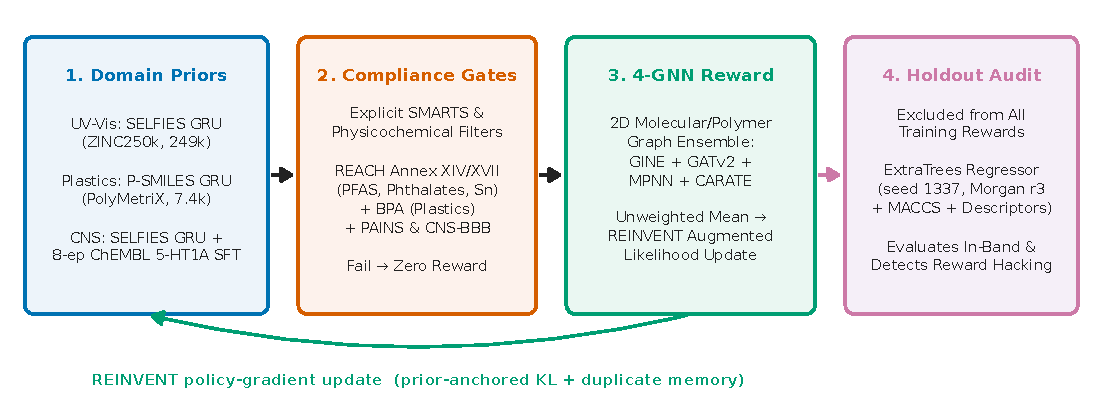
\includegraphics[width=\textwidth]{fig_pipeline.pdf}
\caption{Unified compliance-conditioned generation pipeline across UV-Vis chromophores,
engineering polymers, and central nervous system ligands. Hard regulatory and safety gates
zero the reward of non-compliant candidates before 4-GNN ensemble scoring, while an
independent ExtraTrees holdout audits reward hacking outside the training loop.}
\label{fig:pipeline}
\end{figure}

\section{Results}

\subsection{Track 1: UV-Vis chromophores (400--450~nm)}
Using the public experimental UV-Vis database of Joung et al.~\cite{joung2020uvvis}
(6{,}425 chromophores, $n_{\mathrm{train}}=\MacroUvNtrain{}$, $n_{\mathrm{test}}=\MacroUvNtest{}$),
every GNN outperforms the baseline Morgan-HGB surrogate (\MacroMorganMae{}~nm MAE), and the 4-GNN ensemble reaches
\textbf{\MacroUvEnsMae{}~nm MAE} ($R^2=\MacroUvEnsRsq{}$, Table~\ref{tab:predictors}), beating the ExtraTrees holdout (\MacroUvHoldMae{}~nm).

Table~\ref{tab:uvvis} traces steering progression across three prior seeds ($n=10{,}000$ fresh samples per seed).
Prefix conditioning shifts in-band yield modestly. Round-3 REINVENT with a 60/40 blend of the
4-GNN ensemble and Morgan-HGB raises 4-GNN in-band yield to \MacroUvGnnInband{}, matching the independent ExtraTrees holdout (\MacroUvEtInband{}) with $3.7\times$ lower cross-seed variance than a Morgan-only policy, $0.950$ uniqueness, $1.000$ novelty, and $0.983$ rule pass (Table~\ref{tab:uvvis}).

% Auto-generated — do not edit.
\begin{table}[t]
\centering
\caption{Track 1 (UV-Vis 400--450~nm): in-band fraction $\phi_{[400,450]}$ by audit oracle. Final row: three prior seeds, 10{,}000 samples each (mean $\pm$ SD). Holdout ExtraTrees never enters training rewards.}
\label{tab:uvvis}
\scriptsize
\resizebox{\textwidth}{!}{
\begin{tabular}{@{}lrrrrrrr@{}}
\toprule
Method & Holdout ET & Ens.\ 4-GNN & \texttt{GINE} only & Morgan-HGB & Uniq. & Rule & Int.\ div. \\
\midrule
Plain ZINC250k prior & 0.191 & -- & 0.078 & 0.185 $\pm$ 0.006 & 1.000 & 0.963 & 0.886 \\
Prefix conditioning & 0.231 & -- & -- & 0.252 $\pm$ 0.004 & 1.000 & 0.999 & 0.885 \\
REINVENT Round~2 (\texttt{a29221}) & 0.543$\pm$0.049 & -- & -- & 0.598$\pm$0.015 & 0.986$\pm$0.005 & 0.999$\pm$0.001 & 0.799$\pm$0.012 \\
REINVENT Round~3 (\texttt{403657}, Morgan) & 0.728$\pm$0.093 & -- & 0.514 & 0.512 $\pm$ 0.038 & 0.950 $\pm$ 0.010 & 0.983 $\pm$ 0.004 & 0.799 $\pm$ 0.010 \\
\textbf{REINVENT 4-GNN + Morgan (\texttt{403657})} & \textbf{0.702 $\pm$ 0.025} & \textbf{0.720 $\pm$ 0.037} & -- & 0.512 $\pm$ 0.038 & \textbf{0.950 $\pm$ 0.010} & \textbf{0.983 $\pm$ 0.004} & 0.799 $\pm$ 0.010 \\
\bottomrule
\multicolumn{8}{@{}l}{\footnotesize \texttt{GINE}-only column: $n=3{,}000$, prior seed~1 (\texttt{uvvis\_steering\_progression.json}). Post-hoc 4-GNN ensemble scoring uses the three-seed 10{,}000-sample protocol (\texttt{4gnn\_ensemble\_summary.json}). Validity and novelty are 1.000 across REINVENT runs.}
\end{tabular}
}
\end{table}


Snapshot evaluations every 200 RL steps (Figure~\ref{fig:curves}A) confirm that 4-GNN and independent Holdout ExtraTrees in-band yields rise together from step~0 to step~1{,}200 while uniqueness remains above $0.99$.

\begin{figure}[t]
\centering
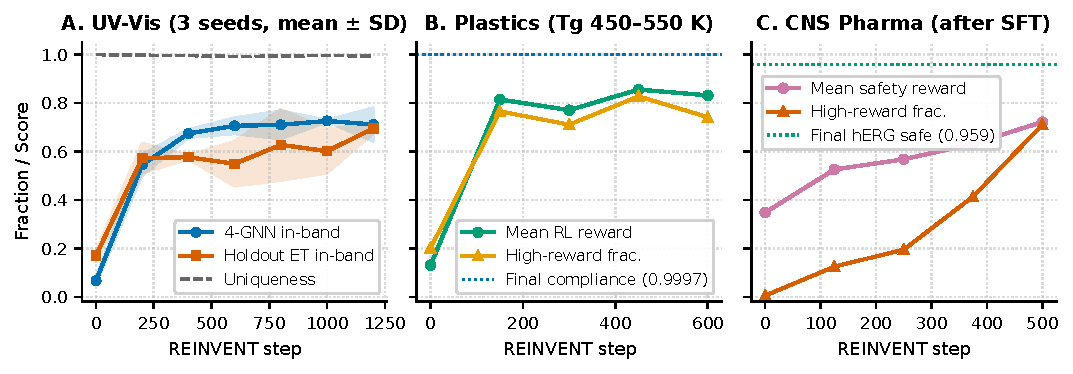
\includegraphics[width=\textwidth]{fig_learning_curves.pdf}
\caption{REINVENT learning curves across all three domains. (A)~UV-Vis 400--450~nm three-seed snapshot trajectory (512 samples per seed every 200 steps, mean $\pm$ SD, $n=3$ seeds). (B)~Plastics ($T_g$ 450--550~K) mean reward and high-reward fraction over 600 RL steps. (C)~CNS multi-objective safety REINVENT over 500 steps following the 8-epoch \texttt{5-HT1A} supervised warm-start.}
\label{fig:curves}
\end{figure}

% Auto-generated — do not edit.
\begin{table}[t]
\centering
\caption{Held-out predictor accuracy across all three domains (90/10 split, GNNs at seed~42, independent Holdout ExtraTrees at seed~1337).}
\label{tab:predictors}
\scriptsize
\resizebox{\textwidth}{!}{
\begin{tabular}{@{}llrrrrrr@{}}
\toprule
Domain / Target & Unit ($n_{\mathrm{test}}$) & \texttt{GINE} & \texttt{GATv2} & \texttt{MPNN} & \texttt{CARATE} & \textbf{4-GNN Ens.\ MAE ($R^2$)} & Holdout ET MAE ($R^2$) \\
\midrule
UV-Vis $\lambda_{\max}$ & nm (643) & 19.64 & 18.35 & 19.86 & 19.84 & \textbf{17.48 (0.922)} & 18.50 (0.928) \\
Polymer $T_g$ & K (737) & 22.10 & 22.88 & 22.86 & 22.56 & \textbf{20.96 (0.922)} & 31.36 (0.818) \\
CNS \texttt{5-HT1A} & pChEMBL (613) & 0.530 & 0.502 & 0.502 & 0.525 & \textbf{0.49 (0.687)} & 0.698 (0.350) \\
Anti-target \texttt{5-HT2B} & pChEMBL (237) & 0.572 & 0.535 & -- & 0.540 & \textbf{0.53 (0.460)}$^a$ & 0.654 (0.094) \\
Anti-target \texttt{hERG} & pChEMBL (1008) & 0.394 & 0.394 & -- & 0.393 & \textbf{0.37 (0.617)}$^a$ & 0.547 (0.286) \\
\bottomrule
\multicolumn{8}{@{}l}{\footnotesize $^a$ 3-GNN ensemble (\texttt{GINE}+\texttt{GATv2}+\texttt{CARATE}). Baseline Morgan-HGB on UV-Vis: 24.04~nm.}
\end{tabular}
}
\end{table}


\subsection{Track 2: Plastics --- REACH- and BPA-free engineering polymers (450--550~K)}
We use the CC-BY-4.0 curated homopolymer $T_g$ dataset of Kunchapu and Jablonka~\cite{kunchapu2025tg}
($N=\MacroCorpN{}$ RDKit-valid P-SMILES). Unlike ZINC250k, this corpus exhibits substantial
regulatory tension: \textbf{\MacroCorpFailPct{}\%} (\MacroCorpFailN{} polymers) fail the combined
REACH+BPA screen. On held-out test polymers ($n=737$), the 4-GNN ensemble achieves
\textbf{\MacroPlEnsMae{}~K MAE} ($R^2=\MacroPlEnsRsq{}$, Table~\ref{tab:predictors}).

After 600 steps of compliance-gated REINVENT targeting $T_g \in [450, 550]$~K
(Table~\ref{tab:plastics}, $n=3{,}000$ samples), P-SMILES validity rises from \MacroPlValidPrior{} to \textbf{\MacroPlValidFinal{}}
and REACH/BPA compliance from \MacroPlCompliancePrior{} to \textbf{0.9997}. In-band yield rises from \MacroPlInbandPriorGnn{} to \textbf{\MacroPlInbandGnn{}} (4-GNN) at $0.926$ uniqueness and $0.991$ novelty.

% Auto-generated
\begin{table}[t]
\centering
\caption{Track 2 (Plastics, $T_g$ 450--550~K, REACH+BPA-free): 3{,}000 fresh P-SMILES samples.}
\label{tab:plastics}
\scriptsize
\resizebox{\textwidth}{!}{
\begin{tabular}{@{}lrrrrrrrr@{}}
\toprule
Model & P-SMILES valid & Compliance & In-band 4-GNN & In-band Holdout & Both+Comp. & Uniq. & Novelty & Int.\ div. \\
\midrule
P-SMILES GRU prior & 0.717 & 0.893 & 0.201 & 0.191 & 0.131 & 0.899 & 0.613 & 0.858 \\
\textbf{Compliance-REINVENT (4-GNN)} & \textbf{0.967} & \textbf{0.9997} & \textbf{0.807} & \textbf{0.522} & \textbf{0.458} & \textbf{0.926} & \textbf{0.991} & 0.674 \\
\bottomrule
\end{tabular}
}
\end{table}


\subsection{Track 3: Pharmaceuticals --- non-hallucinogenic CNS (\texttt{5-HT1A} vs.\ \texttt{5-HT2B} \& \texttt{hERG})}
We extract single-protein pChEMBL records from ChEMBL~37~\cite{zdrazil2024chembl,gaulton2012chembl} for the
non-hallucinogenic psychiatric target \texttt{5-HT1A} (\texttt{CHEMBL214}, 6{,}121 unique
molecules) alongside cardiac safety anti-targets \texttt{5-HT2B} (\texttt{CHEMBL1833}) and
\texttt{hERG} (\texttt{CHEMBL240}). Table~\ref{tab:pharma} reports fractions from $n=3{,}000$
fresh samples per model checkpoint.

Direct RL from the generic ZINC250k prior fails due to reward sparsity. An 8-epoch supervised
warm-start resolves cold-start sparsity but exposes a selectivity trap; smooth additive
multi-objective safety REINVENT without scaffold memory restores cardiac safety metrics yet drops
uniqueness to \MacroCnsUniqSafety{}. Bemis--Murcko caps~\cite{bemis1996murcko} restore uniqueness to
\textbf{\MacroCnsUniqMurcko{}} while maintaining joint all-criteria yield (Table~\ref{tab:pharma}).

% Auto-generated
\begin{table}[t]
\centering
\caption{Track 3 (CNS: \texttt{5-HT1A} $\ge 7.0$, \texttt{5-HT2B} $\le 5.8$, \texttt{hERG} $\le 5.5$, CNS-BBB, REACH/PAINS-free): 3{,}000 fresh samples (reported as fractions; $n=3{,}000$ per row).}
\label{tab:pharma}
\scriptsize
\resizebox{\textwidth}{!}{
\begin{tabular}{@{}lrrrrrrrrr@{}}
\toprule
Model & \texttt{5-HT1A}$\ge 7$ (GNN/ET) & \texttt{5-HT2B}$\le 5.8$ & \texttt{hERG}$\le 5.5$ & CNS-BBB & QED & REACH/PAINS & All (GNN) & Uniq. & Int.\ div. \\
\midrule
ZINC250k prior & 0.001 / 0.244 & 0.565 & 0.859 & 0.667 & 0.658 & 0.939 & 0.0000 & 1.000 & 0.875 \\
SFT warm-start (8 ep.) & 0.351 / 0.487 & 0.179 & 0.608 & 0.502 & 0.566 & 0.974 & 0.0037 & 0.998 & 0.861 \\
Safety-REINVENT (no scaf. mem.) & 0.421 / 0.912 & 0.551 & 0.959 & 0.982 & 0.789 & 0.998 & 0.0217 & 0.266 & 0.603 \\
\textbf{Safety-REINVENT + Murcko mem.} & \textbf{0.445 / 0.507} & \textbf{0.228} & \textbf{0.750} & \textbf{0.788} & \textbf{0.688} & \textbf{0.987} & \textbf{0.0243} & \textbf{0.994} & \textbf{0.852} \\
\bottomrule
\end{tabular}
}
\end{table}


\begin{figure}[t]
\centering
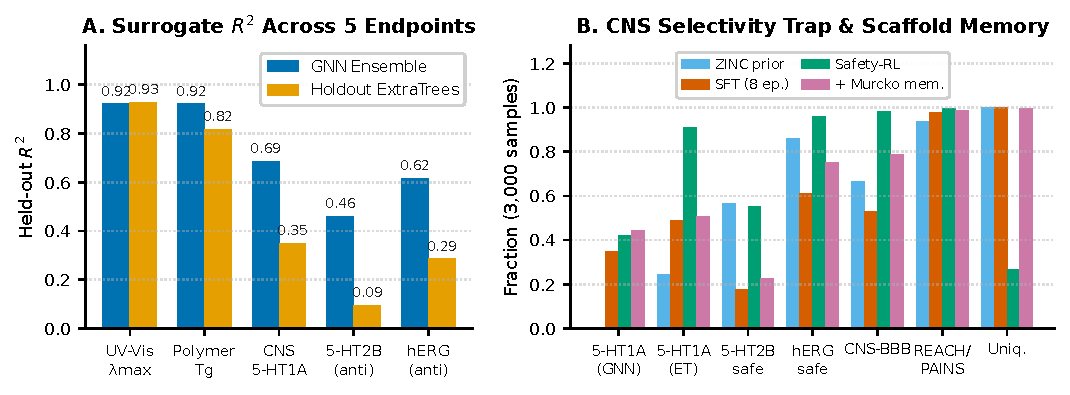
\includegraphics[width=\textwidth]{fig_cross_domain_summary.pdf}
\caption{Cross-domain quantitative summary. (A)~Held-out $R^2$ of the GNN ensembles versus independent ExtraTrees across all five endpoints (Table~\ref{tab:predictors}). (B)~CNS selectivity trap after supervised warm-starting and multi-objective recovery (Table~\ref{tab:pharma}, $n=3{,}000$).}
\label{fig:summary}
\end{figure}

\subsection{Retrosynthetic accessibility and TD-DFT audit}
To assess synthetic tractability beyond string validity, we evaluate Ertl--Schuffenhauer
SA-Score~\cite{ertl2009sa} and RDKit BRICS retrosynthetic disconnection~\cite{degen2008brics}
across all three domains (Table~\ref{tab:retro} and Figure~\ref{fig:dft_retro}B).

To audit surrogate predictions against first-principles quantum chemistry, we sampled $n=50$
novel REACH-compliant UV-Vis consensus candidates ($\le 30$ heavy atoms, all $\mathrm{SA}\le 4.0$),
generated ETKDGv3/MMFF94 3D conformers, and ran gas-phase linear-response time-dependent DFT
(TD-DFT) at the Tamm--Dancoff approximation with the B3LYP exchange-correlation functional and
6-31G split-valence basis set, requesting three singlet roots, using PySCF~\cite{sun2016pyscf}
(Figure~\ref{fig:dft_retro}A). No continuum solvation or vibronic broadening was applied;
excitation energies are vertical gas-phase values appropriate for ranking chromophore plausibility
rather than quantitative spectroscopy. All 46 charge-neutral, basis-supported structures converged
($\MacroDftConvFrac{}\%$ of the 50-molecule pool). Converged candidates exhibit mean
HOMO--LUMO gap $3.36 \pm 0.61$~eV and median $S_1 = 399.4$~nm. Overall, $30/46$ (\MacroDftVisFrac{}\%)
absorb in the visible ($\ge 380$~nm). The \MacroDftMaeGnn{}~nm MAE between 4-GNN and gas-phase $S_1$
quantifies the residual surrogate-to-quantum gap.

% Auto-generated
\begin{table}[t]
\centering
\caption{Retrosynthetic accessibility audit across all three domains (Ertl--Schuffenhauer SA-Score and RDKit BRICS disconnection).}
\label{tab:retro}
\scriptsize
\resizebox{\textwidth}{!}{
\begin{tabular}{@{}lrrrrrr@{}}
\toprule
Domain / Candidate pool & $N$ & SA-Score (mean $\pm$ SD) & $\mathrm{SA} \le 4.0$ & BRICS decomp. & Mean frags & Mean chiral \\
\midrule
UV-Vis (all REACH-compliant) & 592 & $2.92 \pm 0.32$ & 0.988 & 0.993 & 5.45 & 0.04 \\
UV-Vis (TD-DFT audit pool) & 50 & $2.90 \pm 0.17$ & 1.000 & 0.960 & 5.26 & 0.00 \\
Plastics (top compliant, Me-capped) & 50 & $2.48 \pm 0.38$ & 1.000 & 0.980 & 5.66 & 0.02 \\
CNS Pharma (top consensus v3) & 10 & $3.71 \pm 0.53$ & 0.700 & 1.000 & 4.70 & 1.50 \\
\bottomrule
\end{tabular}
}
\end{table}


\begin{figure}[t]
\centering
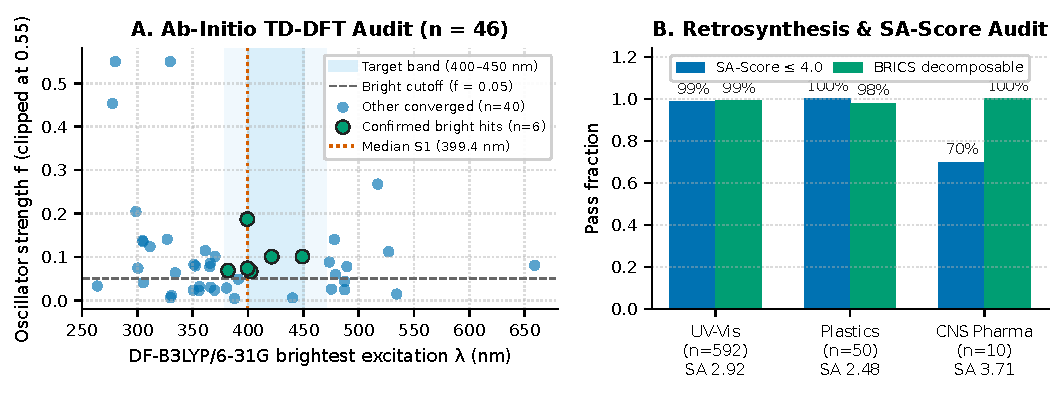
\includegraphics[width=\textwidth]{fig_dft_retrosynth.pdf}
\caption{Post-generation physical and synthetic audits. (A)~Gas-phase B3LYP/6-31G TD-DFT brightest vertical excitation versus oscillator strength across 46 converged UV-Vis candidates (median $S_1 = 399.4$~nm). (B)~SA-Score ($\le 4.0$) and BRICS pass rates across domains (Table~\ref{tab:retro}).}
\label{fig:dft_retro}
\end{figure}

\section{Discussion and Limitations}
Three consistent findings emerge across optical, polymer, and CNS design. Graph ensembles
outperform fingerprint trees on conjugation-sensitive and receptor-binding endpoints; hard
compliance gates reach $>98$--$99.9\%$ pass rates with high target yield; and scaffold-aware RL
recovers uniqueness after multi-objective safety fine-tuning.

Scope boundaries include surrogate versus experimental measurement, SMARTS pattern screens
versus formal regulatory clearance, SA-Score heuristics versus bench synthesis, and the absence
of published-method baselines (REINVENT~4, GraphGA, filter-after-generation) in the present
numeric comparison---runnable scripts and oracle budgets are included for follow-up experiments.

\section*{Data and Software Availability Statement (JCIM)}
All custom code, SMARTS compliance rules, evaluation JSON, and figure-generation scripts are
available at \url{https://github.com/cap-jmk-real/compliance-conditioned-molgen} (commit pinned
in the repository README at submission time). No new experimental raw data were generated.
Public training corpora: ZINC250k~\cite{sterling2015zinc15}, Joung UV-Vis~\cite{joung2020uvvis},
PolyMetriX curated $T_g$~\cite{kunchapu2025tg}, and ChEMBL~37~\cite{zdrazil2024chembl}. Headline
metrics are regenerated from committed result files via
\texttt{paper\_3domain/scripts/generate\_paper\_artifacts.py}; continuous integration executes
\texttt{tests/test\_paper\_generated\_drift.py} to detect manuscript--artifact drift.

\section*{Conflicts of interest}
The author declares no conflict of interest.

\bibliography{refs}

\end{document}